\title{Computational Neurophysiology - Assignment 3}
\author{Ryan Spangler}
\date{\today}

\documentclass[12pt]{article}

\usepackage{commath}
\usepackage{graphicx}

\setcounter{secnumdepth}{0}

\begin{document}
\maketitle

\section{1 - Hodgkin Huxley}

When the potassium current is removed from the Hodgkin Huxley equations and the leak reversal is set to -77 mV, the following behavior occurs, highlighting the dual equilibria in the equation:

\vspace{10pt}
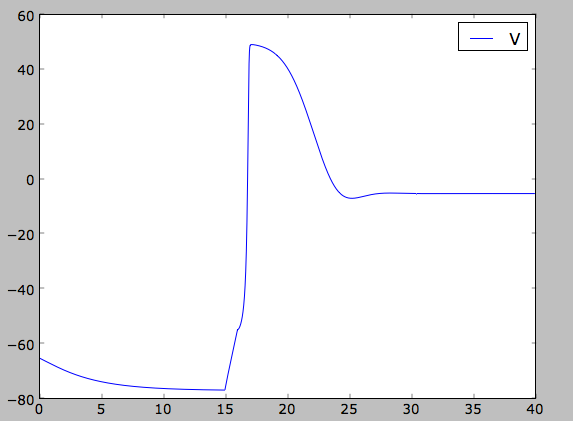
\includegraphics[scale=0.67]{nopotassium.png}

Here, a stimulus was introduced at 15 ms that persisted for 1 ms at an amplitude of 0.3 mV.  Without the stimulus the behavior stays flat at -77 mV, the reversal potential of the leak current.  In order to trigger the spike the potential must rise above -60 mV, where the positive feedback loop of opening sodium channels raising the potential triggering the opening of more sodium channels kicks in.  In this case the spike depolarizes to around 50 mV before settling back to just below 0 mV, a balance struck between the sodium current and the leakage current.  

At the negative leakage equilibrium, $I_Na$ is reduced to basically zero, while $h$ is just under 0.9 and $m$ is just above 0, as is given in the next diagram:

\vspace{10pt}
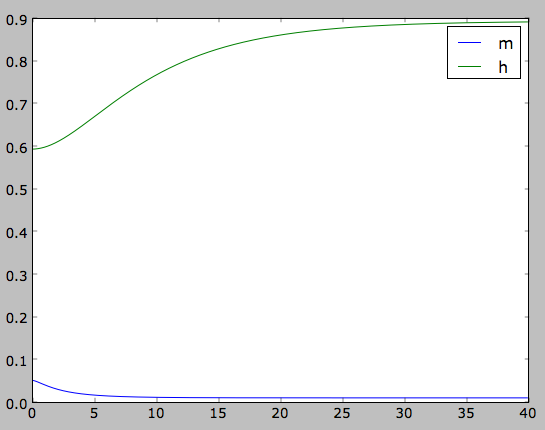
\includegraphics[scale=0.67]{leakequilibrium.png}
\vspace{10pt}

This follows, as $m$ represents the open sodium gates, which do not start opening until the membrane potential passes somewhere above -60 mV.  If the stimulus is applied and the sodium current is allowed to flow, $m$ and $h$ take a different character:

\vspace{10pt}
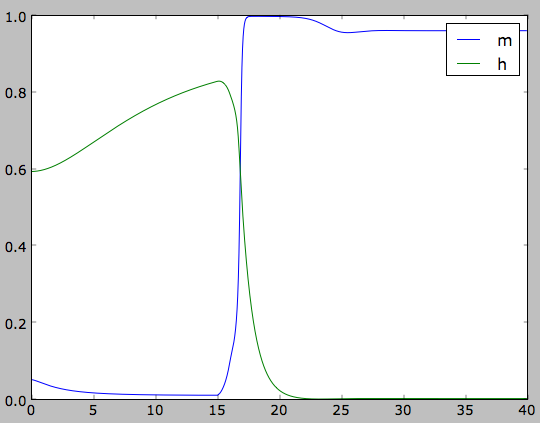
\includegraphics[scale=0.54]{naequilibrium.png}
\vspace{10pt}

Here, as before, the stimulus is applied at $t=15$ ms for 1 ms.  A dramatic change takes place as the $m$ gates open, sodium rushes into the soma and the $h$ inactivation term levels out to 0.  Sodium current has a big flash right at the stimulus point and then levels out to a steady 21.5 uA.  

\vspace{10pt}
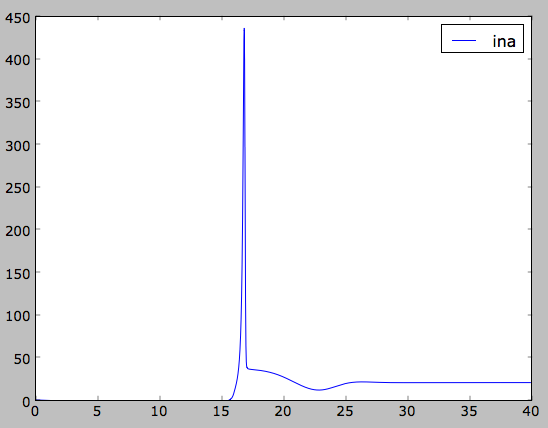
\includegraphics[scale=0.54]{nacurrent.png}
\vspace{10pt}

\section{2 - Post Inhibitory Rebound}

{\bf A)}  Post-inhibitory rebound is made possible by the voltage-dependence of the various gates involved in the action potential.  If one of the sodium gate variables rise in the presence of hyperpolarization, then in effect this is priming the system to make firing more likely than it would be if the hyperpolarization were not experienced.  This is what we see in the case of the $h$ variable.  Under the influence of voltage-clamping at -90 mV with a leak reversal of -54.4 mV, this is the contour of the $m$, $h$ and $n$ variables, corresponding to sodium activation, sodium inactivation and potassium activation respectively:

\vspace{10pt}
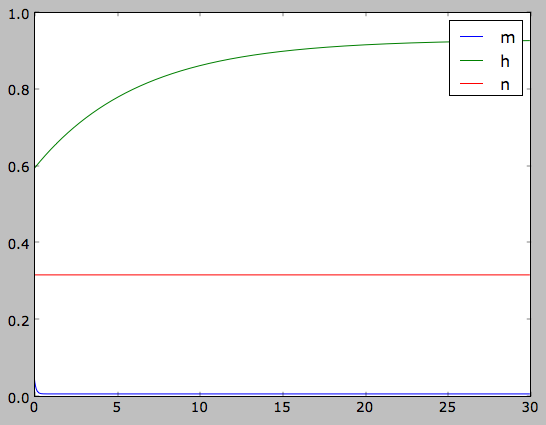
\includegraphics[scale=0.59]{risingh.png}
\vspace{10pt}

Here, while $m$ and $n$ stay level at 0.008 and 0.318 respectively, $h$ rises from its initial value of 0.595 to above 0.9.  This sets the stage for a later spike:

\vspace{10pt}
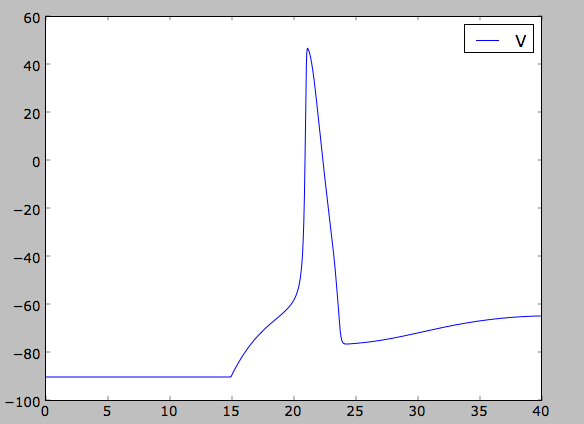
\includegraphics[scale=0.54]{hyperspike.png}
\vspace{10pt}

The voltage clamp is applied for 15 ms at -90 mV, then released.  There is no stimulus present, and yet the spike still occurs.  This is due to the hyperpolarization raising the level of $h$, encouraging spiking.

Here is the behavior of $m$, $h$, and  $n$ over the same time period:

\vspace{10pt}
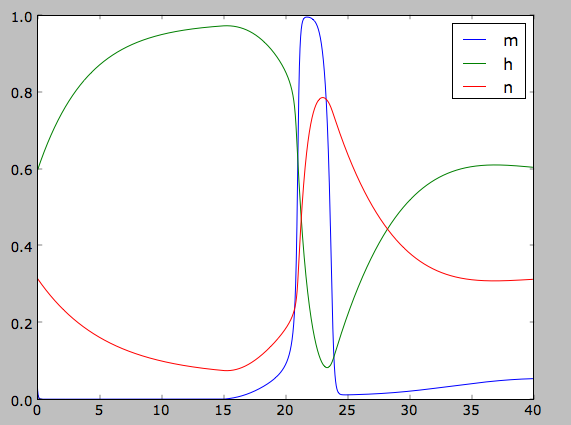
\includegraphics[scale=0.54]{mhnhyper.png}
\vspace{10pt}

The thing to note about this figure is the behavior of $h$, in green.  It rises during the period of depolarization, making it more likely that a spike will occur.

Compare to the exact same system with a stimulus without the period of clamped hyperpolarization (here the stimulus happens at $t=5$ ms):

\vspace{10pt}
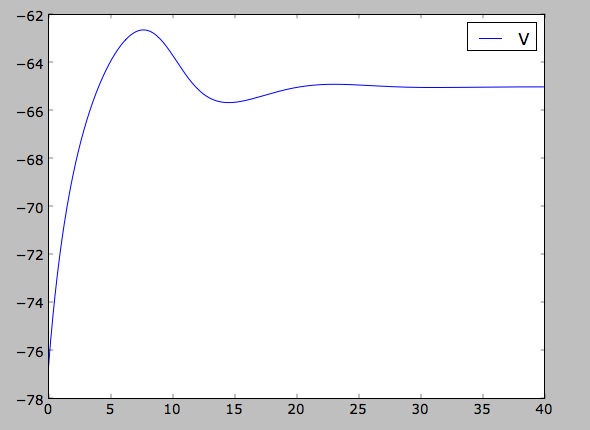
\includegraphics[scale=0.41]{nonhypernonspike.png}
\vspace{10pt}

Here the potential never passes the threshhold even though the stimulus is identical.  $h$ was not experiencing pressure to rise from a hyperpolarized potential and never rose sufficient level to allow the stimulus to trigger the spike, as can be seen in the following figure where all three of the values fall into a smooth equilibrium, $h$ hovering right around 5.95:

\vspace{10pt}
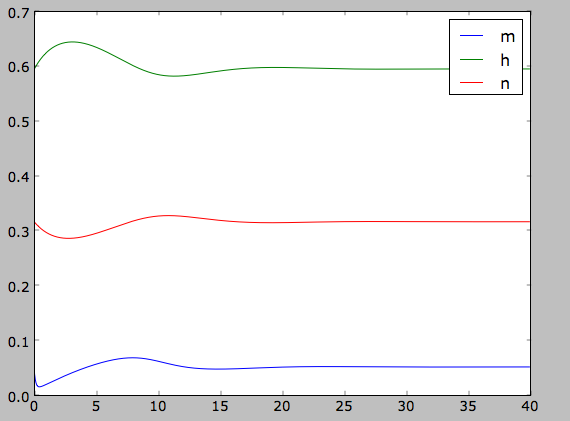
\includegraphics[scale=0.41]{mhnnonhyper.png}
\vspace{10pt}

{\bf B)}  In the presence of a $GABA_\alpha$ synapse with current due to chlorine ions which is assumed to have fired at $t=0$, the model exhibits PIR.  Here is a trial with $V_L=54.4$, $V_{Cl^-}=-89$, $\tau_\alpha=1.0$ and $g_\alpha=10$.  

\vspace{10pt}
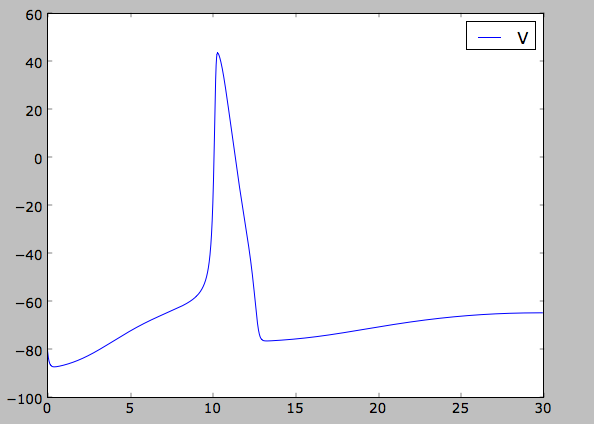
\includegraphics[scale=0.54]{gaba.png}
\vspace{10pt}

The effect of the $GABA_\alpha$ synapse is felt right at the beginning, hyperpolarizing the cell towards the chlorine reversal potential.  As the current from the synapse decays, the potential rises back to the leak reversal, but now armed with a rise in $h$ the hyperpolarization leads to a spike.

\section{3 - Nernst potentials}

{\bf A)}  The Nernst potential for typical concentrations of calcium, which here are $[Ca^{2+}]_{in}=10^{-4}$ mM and $[Ca^{2+}]_{out}=2.1$ mM as measured in the giant squid axon, is:

$$ E_{Ca}=12.5\cdot\ln\frac{2.1}{10^{-4}}=95.62 $$

{\bf B)}  For one variety of ion, the Goldman Hodgkin Katz equation reduces to the Nernst equation.  They are therefore identical when considered with only $Ca^{2+}$.

{\bf C)}  Assume the NMDA channel increases the calcium concentration inside the cell by an order of magnitude, to $10^{-3}$ mM.  This quantity of calcium ions would also be removed from the outside of the cell, making the Nernst equation for these concentrations now

$$ E_{Ca}=12.5\cdot\ln\frac{2.091}{10^{-3}}=66.785 $$

A reduction in potential of almost 30 mV.

\section{4 - Cable properties}



\section{5 - Compartmental models}



\end{document} 
